% !TEX root = ../../1-te.tex

\tocheck{3}{Aktuelle Musterstudienpläne der FG einfügen}
\label{musterstudienplan}

\iftoggle{winter}{
	\begin{minipage}[H]{1.0\linewidth}
	\begin{center}
	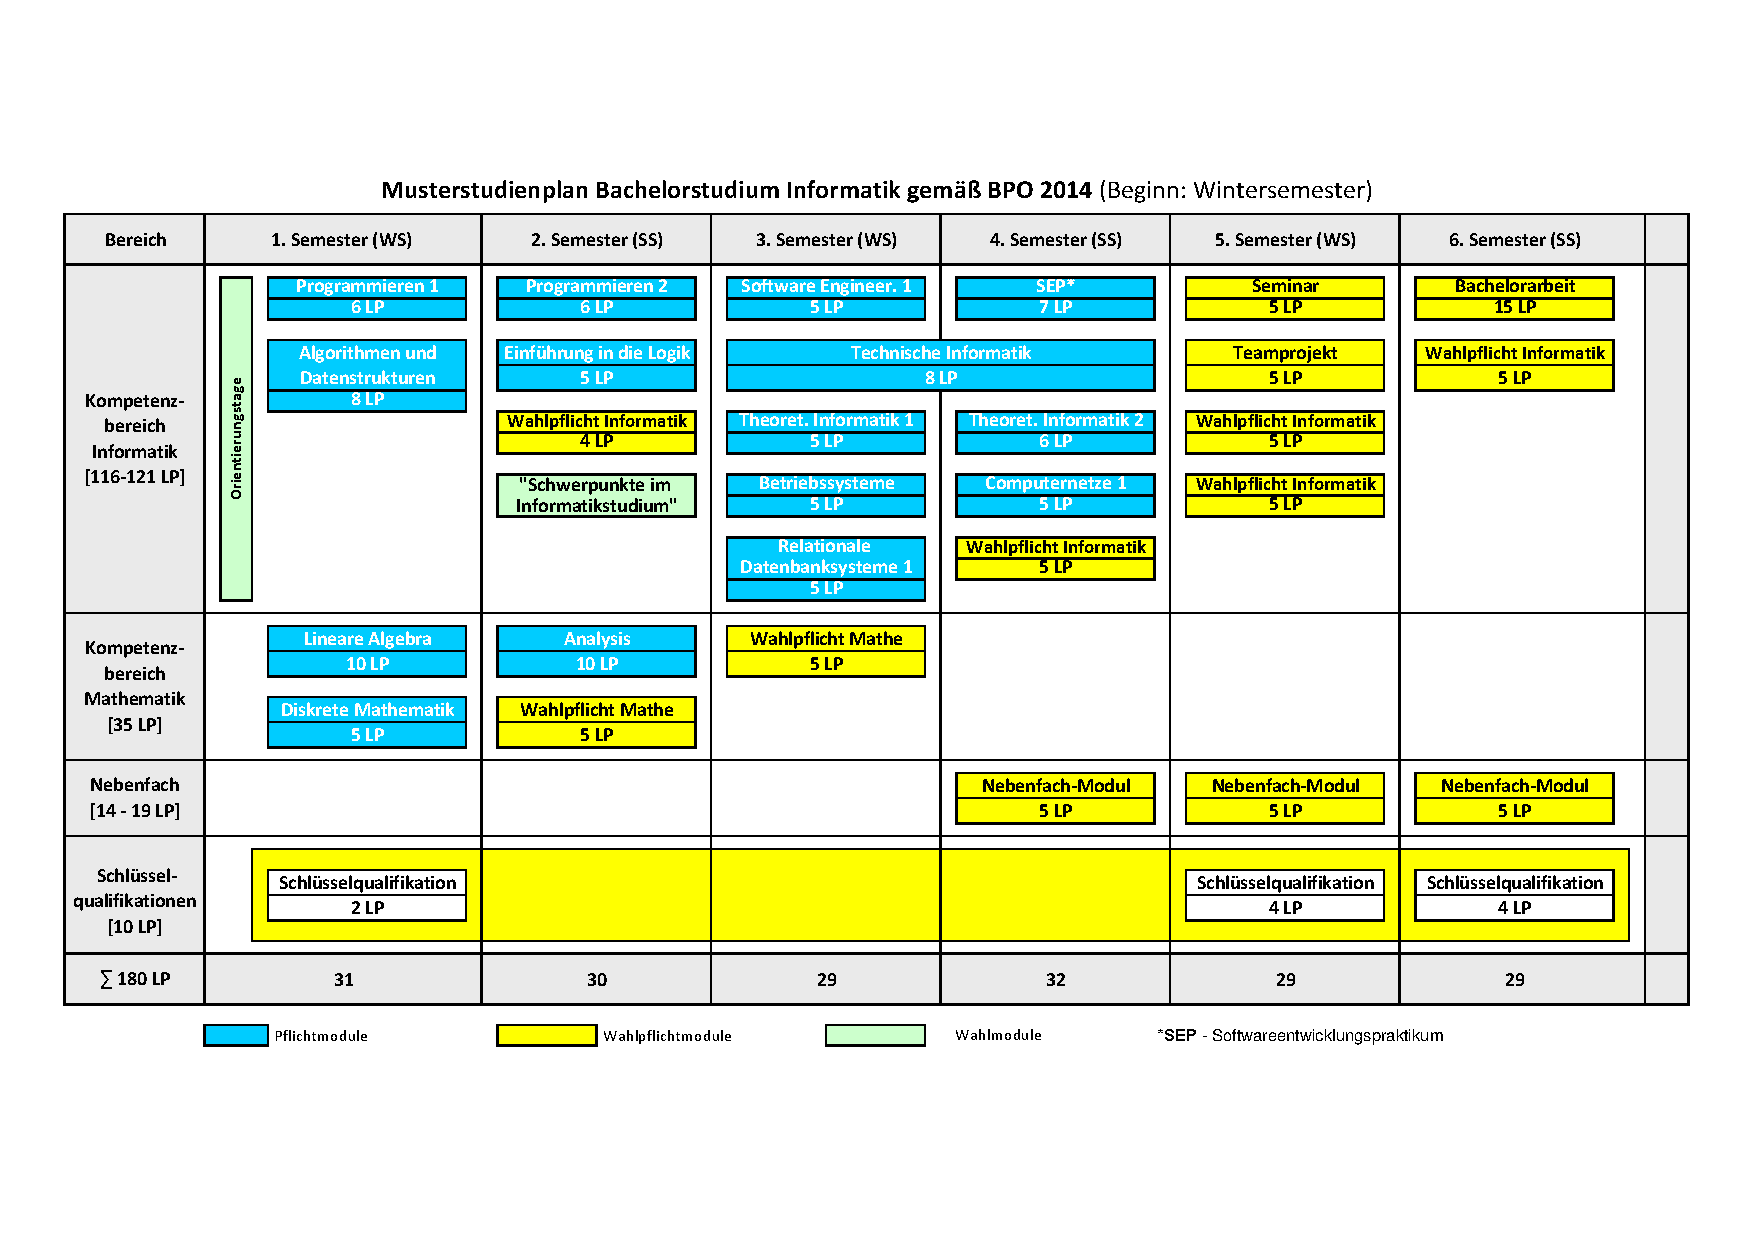
\includegraphics[angle=90, totalheight=\textheight, width=\textwidth ]{bilder/studienplan_bsc_ws/musterstudienplan_ba_neu_abss2014_ws.pdf}
	\end{center}  
	\end{minipage}
	\newpage

	\begin{minipage}[H]{1.0\linewidth}
	\begin{center} 
			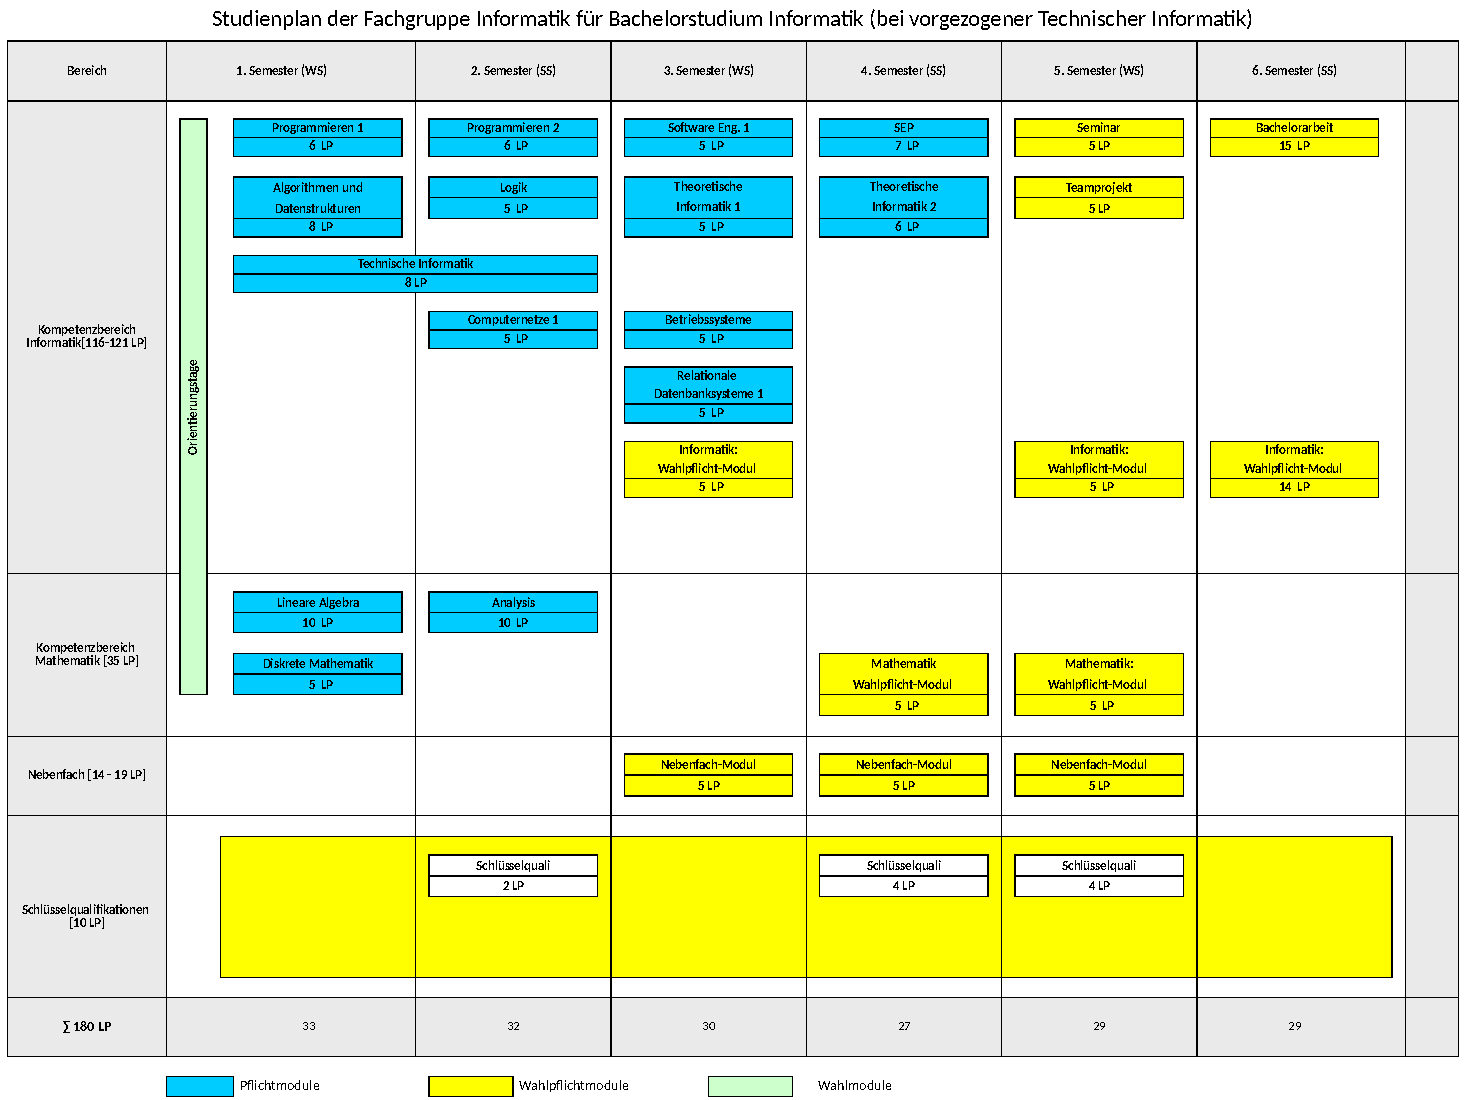
\includegraphics[angle=90, height=\textheight, width=\textwidth ]{bilder/studienplan_bsc_ws/ws2015/BScInformatikWS1516-fginfo-tech_scissored}
			\label{studienplan_tech}
	\end{center}
	\end{minipage}
	\newpage

	\begin{minipage}[H]{1.0\linewidth}
	\begin{center} 
			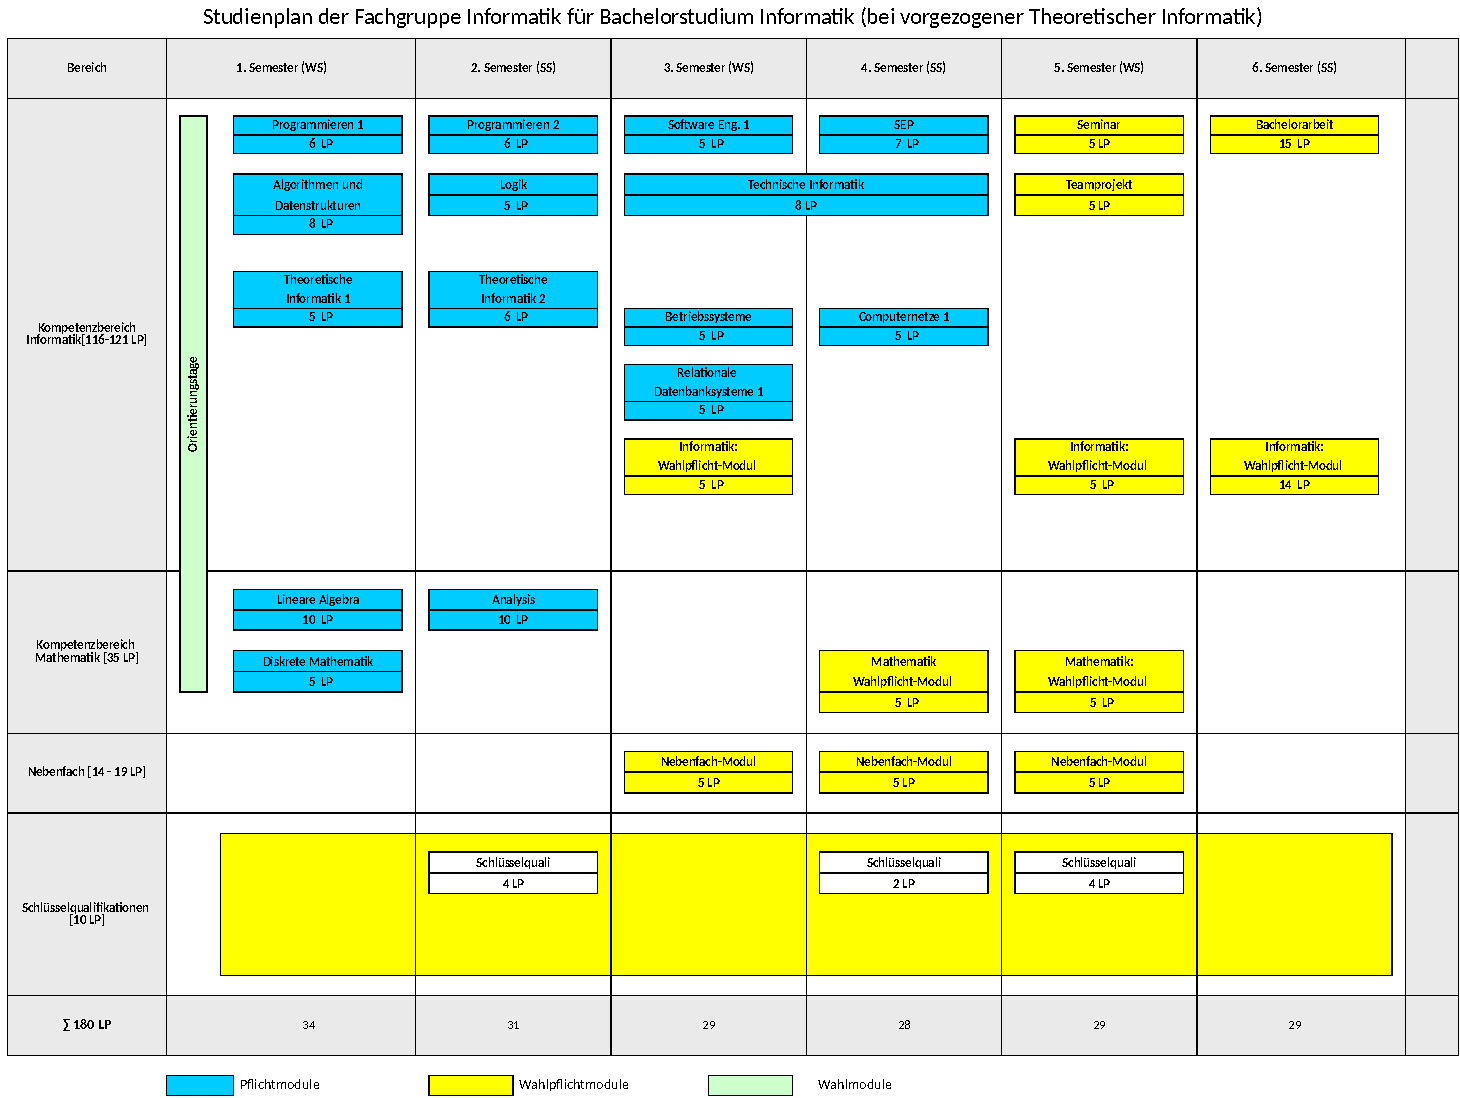
\includegraphics[angle=90, totalheight=\textheight, width=\textwidth ]{bilder/studienplan_bsc_ws/ws2015/BScInformatikWS1516-fginfo-theo_scissored}
			\label{studienplan_theo}
	\end{center}
	\end{minipage}
}{
	\begin{minipage}[H]{1.0\linewidth}
		\begin{center}
		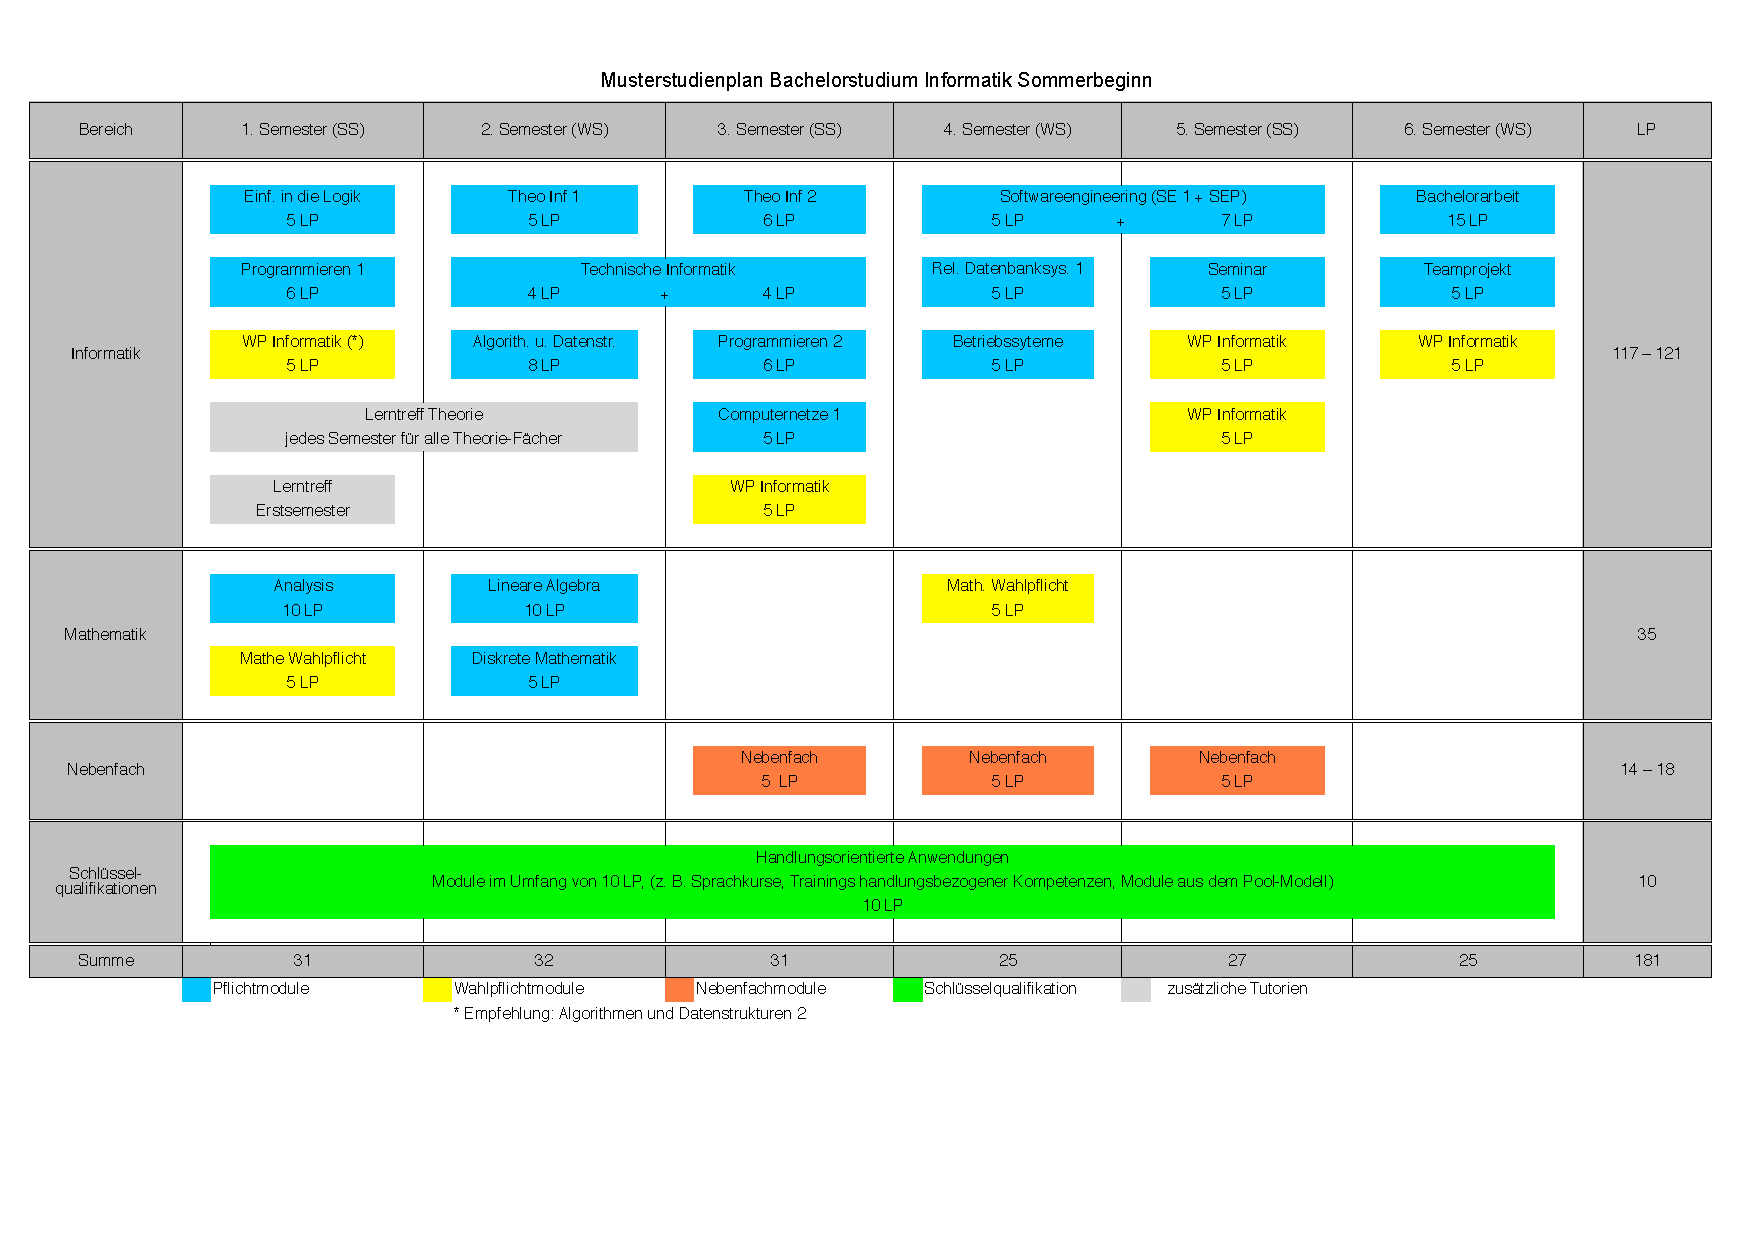
\includegraphics[angle=90, totalheight=\textheight]{bilder/studienplan_bsc_ss/Musterstudienplan_SoSe16.pdf}
		\end{center}  
	\end{minipage}

	\begin{minipage}[H]{1.0\linewidth}
		\begin{center}     
		\label{musterstudienplan}
		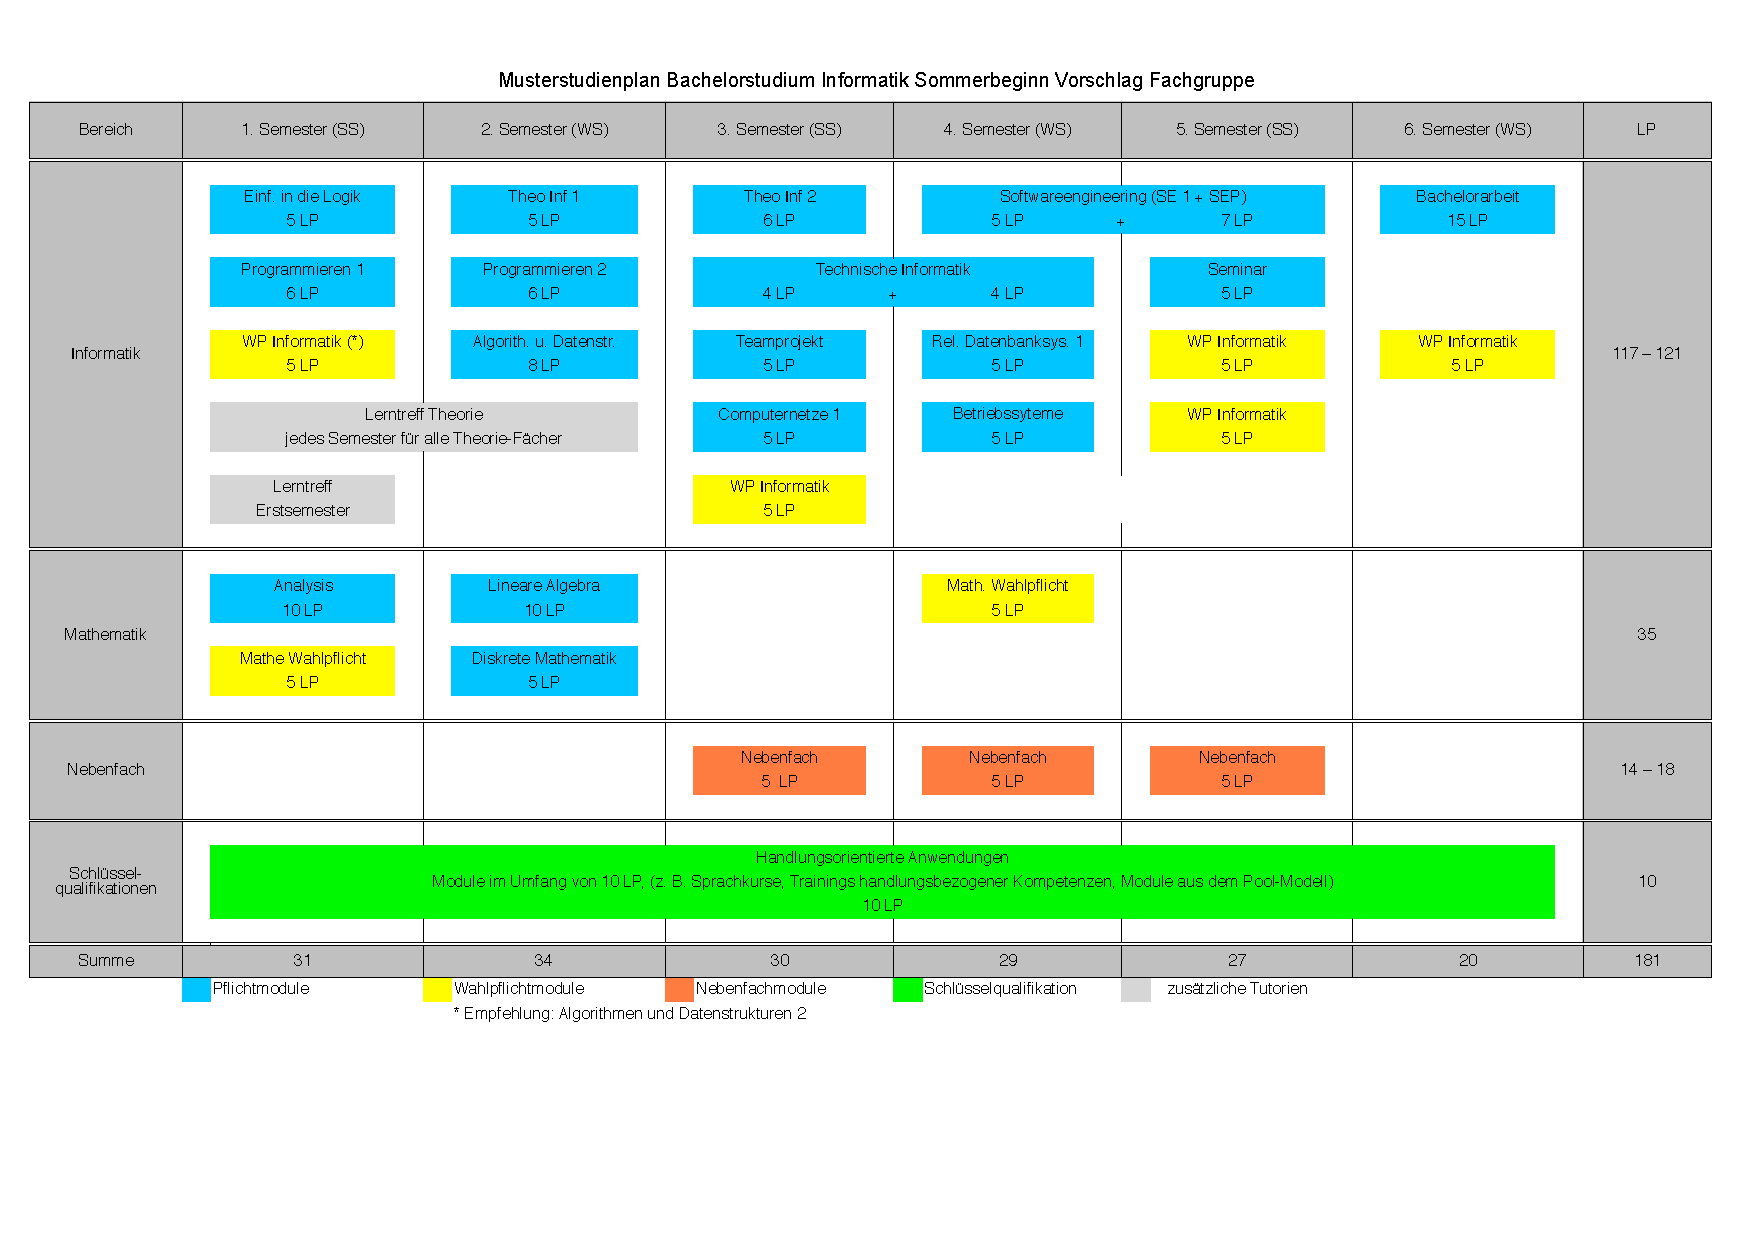
\includegraphics[angle=90, totalheight=\textheight]{bilder/studienplan_bsc_ss/Musterstudienplan_SoSe16_Empfehlung_FG.pdf}
		\end{center}  
	\end{minipage}
}
